\documentclass[12pt]{article}

\usepackage{cite}
\usepackage{amsmath,amssymb,amsfonts}
\usepackage{algorithmic}
\usepackage{graphicx}
\usepackage{textcomp}
\usepackage{xcolor}
\usepackage{float}
\usepackage{subfigure}
\usepackage{listings}
\usepackage{color}

\begin{document}

\title{\textbf{Introduction to Deep Learning Final Report}}
\author{Jin Xu \and Runlin Hou}    
\maketitle


\section{Introduction}
The topic our team chooses is that manually implement a fully-connected NN using Numpy. And 
we finally implement a four-layer fully connected neural network. According to the requirement, 
we are training this model on the MNIST dataset and get accuracy above 90\% at around 200 
epoch.

\section{Dataset}
The dataset we are using is MNIST. This is a large dataset of handwritten digits from 0-9 that 
is commonly used for training various image processing systems. And these numbers are from 250 
different people, which 50\% of them are middle school students, and 50\% of them are faculty 
of the Census Bureau. The dataset itself is divided into a training set that has 60000 samples, 
and a testing set has 10000 samples.  Each image in this dataset has 28x28 pixels. So in the 
training process, we will falt each image into a 784 dimension vector.

\section{Model}
As mentioned in the last section, we build a four-layer network. Considering the image data will be taken, the first layer has 784 neurons and will output 200 neurons. The two hidden layers have 200 and 10 dimensions, respectively.
\begin{center}
    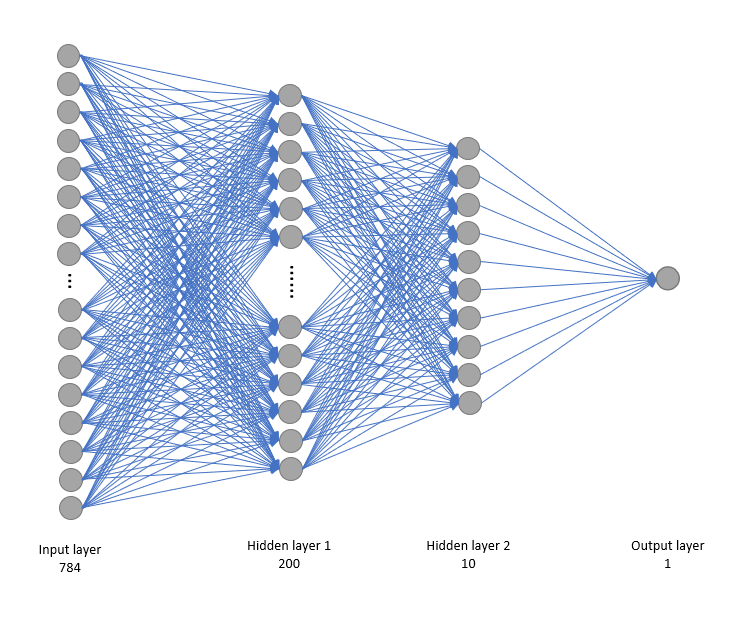
\includegraphics[scale=0.7]{network.png}
\end{center}

\section{Methods}
\subsection*{ReLU}
For ReLU we choose to use the Ramp function, which is a widely used rectifier in the machine 
learning field. As its name showed, the graph of ramp function looks like a ramp. And can be 
described mathematically as follow:
\begin{equation*}
    R(x):=max(0,x)
\end{equation*}

The backward computaion can be seen as:
\begin{equation*}
    \frac{dr_i}{dx_i}=\left\{
        \begin{aligned}
            &0, x_i\leq 0\\
            &1, x_i> 0
        \end{aligned}
    \right.
\end{equation*}

\subsection*{Softmax}
The softmax function takes as input a vector of k real numbers and normalizes it into a probability distribution consisting of K probabilities proportional to the exponentials of the input numbers.
And it can be mathematically defined as follow:
\begin{equation*}
    \sigma(z)_i = \frac{e^{z_i}}{\sum_{j=i}^K e^{z_i}}
\end{equation*}

\subsection*{Loss Function}
We choose to use cross-entropy as our loss function:
\begin{equation*}
    H(p,q) = -\sum_{i=1}^n p(x_i)log(q(x_i))
\end{equation*}

\section{Result}
As we can see from the graph, the accuracy raise rapidly from epoch 0 to 80 and slow down after 
the accuracy reaches 80\%. And also we can see that the accuracy reach above 90\% at around 200
 epoch. However, since we initiate the weights and bias randomly, the process might be much 
 slower if we got bad luck and initiate a series of bad weights.
 \begin{center}
     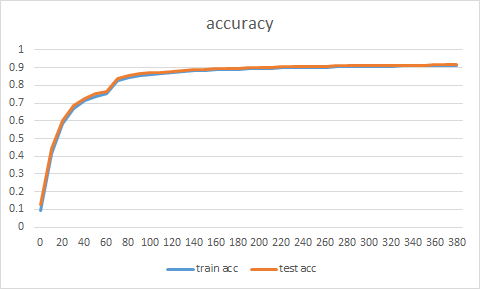
\includegraphics[scale=1]{accuracy.png}
 \end{center}



\end{document}